\chapter{背景}
\label{chap:background}

本章では、研究の背景となったモバイルデバイスの普及、

\newpage
\section{モバイルデバイスの普及}

今日、日本に置いて
スマートフォンやタブレットなどのモバイルデバイスが普及している。
\cite{mobiledevicespread}
総務省による「平成25年通信利用動向調査」によると(図:)
\begin{figure}
  \begin{center}
    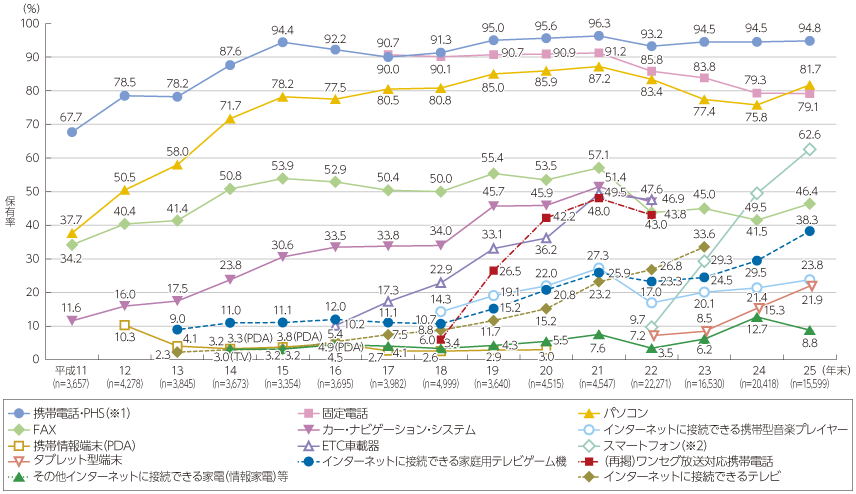
\includegraphics[width=14cm,bb=0 0 856 494]{images/mobiledevicespread.png}
    \caption{主な情報通信機器の普及状況\cite[出典]{communicationreport}}
    \label{mobiledevicespread}
  \end{center}
\end{figure}

現在、
これらのモバイルデバイスを使う上で日本語の入力は欠かすことができない操作である。
デバイスの性能は携帯電話の頃から劇的に向上している。
パソコンに遜色ないようなメモリやCPUを積んでいるものも多く市販されている。
しかし文字入力に関してはあまり成長していない。

文字入力にもデバイスに適したよりよいものがある。
文字入力のユーザの体験ももっと向上すべきである。
今回は日本人向けのシステムとして作った。

ユーザにはそれぞれコンテキストがある。
コンテキストによって入力したい単語は推測できるのではないか

\section{文字入力の歴史}

\section{文字入力への問題点と期待}

スマートウォッチやグーグルグラスなどでは文字入力めんどい
